\documentclass{beamer}

 \pdfmapfile{+sansmathaccent.map}


\mode<presentation>
{
  \usetheme{Warsaw} % or try Darmstadt, Madrid, Warsaw, Rochester, CambridgeUS, ...
  \usecolortheme{crane} % or try seahorse, beaver, crane, wolverine, ...
  \usefonttheme{serif}  % or try serif, structurebold, ...
  \setbeamertemplate{navigation symbols}{}
  \setbeamertemplate{caption}[numbered]
} 

\renewcommand{\familydefault}{\rmdefault}


\hypersetup{
    colorlinks=true,
    linkcolor=blue,
    filecolor=blue,      
    urlcolor=blue,
}

\usepackage{amsmath}
\usepackage{mathtools}

\DeclareMathOperator*{\argmin}{arg\,min}

\usepackage{subcaption}

\usepackage{tikz}
\tikzset{every picture/.style={line width=0.75pt}} %set default line width to 0.75pt        
%%%%%%%%%%%%%%%%%%%%%%%%%%%%%%%%%%%%%%%%%%%%%%%%%%%


\usepackage{listings}
\usepackage{color}
\definecolor{mygreen}{rgb}{0,0.6,0}
\definecolor{mygray}{rgb}{0.5,0.5,0.5}
\definecolor{mymauve}{rgb}{0.58,0,0.82}

\definecolor{cof}{RGB}{255,187,0}
\definecolor{pur}{RGB}{205,137,0}
\definecolor{greeo}{RGB}{91,173,69}
\definecolor{greet}{RGB}{52,111,72}

\usetikzlibrary{fadings}
\usetikzlibrary{patterns}
\usetikzlibrary{shadows.blur}
\usetikzlibrary{shapes}

\lstset{ 
  backgroundcolor=\color{white},   % choose the background color; you must add \usepackage{color} or \usepackage{xcolor}; should come as last argument
  basicstyle=\footnotesize,        % the size of the fonts that are used for the code
  breakatwhitespace=false,         % sets if automatic breaks should only happen at whitespace
  breaklines=true,                 % sets automatic line breaking
  captionpos=b,                    % sets the caption-position to bottom
  commentstyle=\color{mygreen},    % comment style
  deletekeywords={...},            % if you want to delete keywords from the given language
  escapeinside={\%*}{*)},          % if you want to add LaTeX within your code
  extendedchars=true,              % lets you use non-ASCII characters; for 8-bits encodings only, does not work with UTF-8
  firstnumber=0000,                % start line enumeration with line 0000
  frame=single,	                   % adds a frame around the code
  keepspaces=true,                 % keeps spaces in text, useful for keeping indentation of code (possibly needs columns=flexible)
  keywordstyle=\color{blue},       % keyword style
  language=Octave,                 % the language of the code
  morekeywords={*,...},            % if you want to add more keywords to the set
  numbers=left,                    % where to put the line-numbers; possible values are (none, left, right)
  numbersep=5pt,                   % how far the line-numbers are from the code
  numberstyle=\tiny\color{mygray}, % the style that is used for the line-numbers
  rulecolor=\color{black},         % if not set, the frame-color may be changed on line-breaks within not-black text (e.g. comments (green here))
  showspaces=false,                % show spaces everywhere adding particular underscores; it overrides 'showstringspaces'
  showstringspaces=false,          % underline spaces within strings only
  showtabs=false,                  % show tabs within strings adding particular underscores
  stepnumber=2,                    % the step between two line-numbers. If it's 1, each line will be numbered
  stringstyle=\color{mymauve},     % string literal style
  tabsize=2,	                   % sets default tabsize to 2 spaces
  title=\lstname                   % show the filename of files included with \lstinputlisting; also try caption instead of title
}




%%%%%%%%%%%%%%%%%%%%%%%%%%%%%%%%%%%%%%%%%%%%%%%%%%%%%


\title{Linear Programming}
\subtitle{Computational Intelligence, Lecture 9}
\author{by Sergei Savin}
\centering
\date{Fall 2020}



\begin{document}
\maketitle


\begin{frame}{Content}

\begin{itemize}
\item Linear Programming
\begin{itemize}
    \item General form
    \item LP with no solution - examples
\end{itemize}
\item Convex piece-wise linear functions
\begin{itemize}
    \item Problem statement
    \item Solution as LP
    \item Sum of piece-wise linear functions
    \item Code example
\end{itemize}
\item Chebyshev center of a polyhedron
\begin{itemize}
    \item Problem statement
    \item Solution as LP
    \item Code example
\end{itemize}
\item Homework
\end{itemize}

\end{frame}



\begin{frame}{Linear Programming}
\framesubtitle{General form}
\begin{flushleft}

A linear program (LP) is an optimization problem of the form:

\begin{equation} \label{LP}
\begin{aligned}
& \underset{\mathbf{x}}{\text{minimize}}
& & \mathbf{f}^\top \mathbf{x} , \\
& \text{subject to}
& & \begin{cases} 
\mathbf{A}\mathbf{x} \leq \mathbf{b}, \\
\mathbf{C}\mathbf{x} = \mathbf{d}.
\end{cases}
%
\end{aligned}
\end{equation}

It is one of the older and widely used classes of convex optimization problems. 

\bigskip

Note that the solution of such problem will always lie on the boundary of its domain.
 
\end{flushleft}
\end{frame}




\begin{frame}{Linear Programming}
\framesubtitle{LP with no solution - examples}
\begin{flushleft}

Here are some examples of LP which have no solutions:

\begin{equation}
\begin{aligned}
& \underset{\mathbf{x}}{\text{minimize}}
& & \begin{bmatrix} 1 & 1 \end{bmatrix} 
\begin{bmatrix} x_1 \\ x_2 \end{bmatrix}
\end{aligned}
\end{equation}

This one is has no boundaries at all, hence no solution. Next one has boundaries, but they do not restrict motion along the descent direction for the cost function.

\begin{equation}
\begin{aligned}
& \underset{\mathbf{x}}{\text{minimize}}
& & \begin{bmatrix} 1 & 1 \end{bmatrix} 
\begin{bmatrix} x_1 \\ x_2 \end{bmatrix} , \\
& \text{subject to}
& & \begin{bmatrix} 1 & 0 \end{bmatrix}
\begin{bmatrix} x_1 \\ x_2 \end{bmatrix} \leq
1
%
\end{aligned}
\end{equation}

 
\end{flushleft}
\end{frame}



\begin{frame}{Convex piece-wise linear functions}
\framesubtitle{Problem statement}
\begin{flushleft}

Convex piece-wise linear functions have the form:

\begin{equation}
    f(\mathbf{x}) = \text{max}(\mathbf{a}_i^\top \mathbf{x} + b_i)
\end{equation}

Figure below shows geometric interpretation of such function for a one-dimensional case.

\begin{figure} [h!]
\begin{center}

\tikzset{every picture/.style={line width=0.75pt}} %set default line width to 0.75pt        

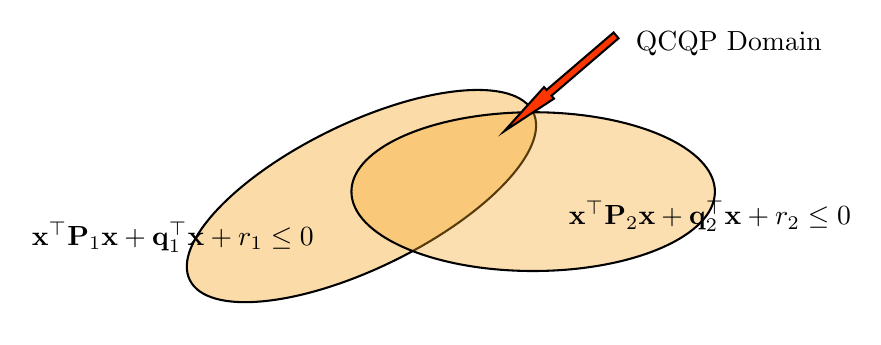
\begin{tikzpicture}[x=0.75pt,y=0.75pt,yscale=-0.75,xscale=0.75]
%uncomment if require: \path (0,300); %set diagram left start at 0, and has height of 300

%Shape: Ellipse [id:dp9898126968799086] 
\draw  [fill={rgb, 255:red, 245; green, 166; blue, 35 }  ,fill opacity=0.4 ] (103.44,199.35) .. controls (92.18,176.27) and (132.43,133.45) .. (193.35,103.71) .. controls (254.27,73.97) and (312.79,68.57) .. (324.06,91.65) .. controls (335.32,114.73) and (295.07,157.55) .. (234.15,187.29) .. controls (173.23,217.03) and (114.71,222.43) .. (103.44,199.35) -- cycle ;
%Shape: Ellipse [id:dp5973223095827915] 
\draw  [fill={rgb, 255:red, 245; green, 166; blue, 35 }  ,fill opacity=0.36 ] (207.31,142.65) .. controls (207.31,114.48) and (259.58,91.65) .. (324.06,91.65) .. controls (388.54,91.65) and (440.81,114.48) .. (440.81,142.65) .. controls (440.81,170.82) and (388.54,193.65) .. (324.06,193.65) .. controls (259.58,193.65) and (207.31,170.82) .. (207.31,142.65) -- cycle ;
%Left Arrow [id:dp11071847750004182] 
\draw  [fill={rgb, 255:red, 255; green, 53; blue, 0 }  ,fill opacity=1 ] (305.5,103.83) -- (331.05,75.5) -- (332.64,77.36) -- (375.73,40.44) -- (378.91,44.15) -- (335.82,81.07) -- (337.41,82.92) -- cycle ;

% Text Node
\draw (0,160) node [anchor=north west][inner sep=0.75pt]    {$\mathbf{x}^\top \mathbf{P}_1 \mathbf{x} + \mathbf{q}_1^\top\mathbf{x} + r_1 \leq 0$};
% Text Node
\draw (345,147) node [anchor=north west][inner sep=0.75pt]    {$\mathbf{x}^\top \mathbf{P}_2 \mathbf{x} + \mathbf{q}_2^\top\mathbf{x} + r_2 \leq 0$};
% Text Node
\draw (388,38) node [anchor=north west][inner sep=0.75pt]   [align=left] {QCQP Domain};


\end{tikzpicture}

\end{center} 
% \caption{Visualization of trajectory generation done in the developed software}
\end{figure}

 
\end{flushleft}
\end{frame}




\begin{frame}{Convex piece-wise linear functions}
\framesubtitle{Solution as LP}
\begin{flushleft}

We can formulate a minimization problem using convex piece-wise linear functions:

\begin{equation}
\begin{aligned}
& \underset{\mathbf{x}}{\text{minimize}}
& & \text{max}(\mathbf{a}_i^\top \mathbf{x} + b_i)
\end{aligned}
\end{equation}

\bigskip

Which can be equivalently transformed into the following LP:

\begin{equation}
\begin{aligned}
& \underset{\mathbf{x}}{\text{minimize}}
& & t \\
& \text{subject to}
& & \mathbf{a}_i^\top \mathbf{x} + b_i \leq t
%
\end{aligned}
\end{equation}

We can observe that optimal (minimal) $t$ will have to lie on one of the linear functions $\mathbf{a}_i^\top \mathbf{x} + b_i$, i.e. on the original piece-wise linear function $f(\mathbf{x})$. And optimal value on t corresponds to the smallest value of the original function $f(\mathbf{x})$.
 
\end{flushleft}
\end{frame}



\begin{frame}{Sum of piece-wise linear functions}
\framesubtitle{Solution as LP}
\begin{flushleft}


Sum of convex piece-wise linear functions have the form:

\begin{equation}
    f(\mathbf{x}) + g(\mathbf{x}) = \text{max}(\mathbf{a}_i^\top \mathbf{x} + b_i) +  \text{max}(\mathbf{c}_i^\top \mathbf{x} + d_i)
\end{equation}

\bigskip

Their representation as LP is:

\begin{equation}
\begin{aligned}
& \underset{\mathbf{x}}{\text{minimize}}
& & t_1 + t_2 \\
& \text{subject to}
& & \begin{cases}
\mathbf{a}_i^\top \mathbf{x} + b_i \leq t_1 \\
\mathbf{c}_i^\top \mathbf{x} + d_i \leq t_2
\end{cases}
%
\end{aligned}
\end{equation}


 
\end{flushleft}
\end{frame}




\begin{frame}{Convex piece-wise linear functions}
\framesubtitle{Code}
\begin{flushleft}

\begin{lstlisting}[language=Matlab]
n = 2;
shift_1 = 1*rand(n, 1);
shift_2 = 1*rand(n, 1);
V1 = randn(n, 6);
V2 = randn(n, 6) + shift_1;
V3 = randn(n, 6) + shift_1 + shift_2;

indices_convhull = convhull(V1');
V1 = V1(:, indices_convhull);
indices_convhull = convhull(V2');
V2 = V2(:, indices_convhull);
indices_convhull = convhull(V3');
V3 = V3(:, indices_convhull);

[A1, b1] = vert2con(V1');
[A2, b2] = vert2con(V2');
[A3, b3] = vert2con(V3');
\end{lstlisting}
 
\end{flushleft}
\end{frame}



\begin{frame}{Chebyshev center of a polyhedron}
\framesubtitle{Problem statement}
\begin{flushleft}

Chebyshev center of a polyhedron is the center of the largest ball inscribed in a polyhedron:

\begin{figure} [h!]
\begin{center}

% \tikzset{every picture/.style={line width=0.75pt}} %set default line width to 0.75pt        

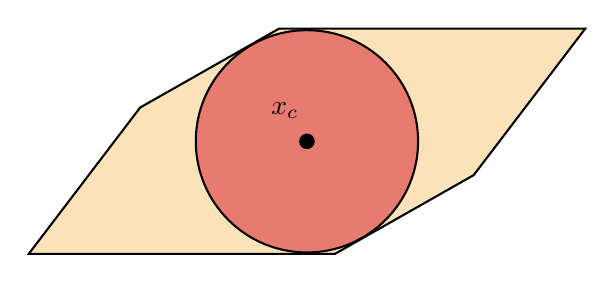
\begin{tikzpicture}[x=0.75pt,y=0.75pt,yscale=-0.7,xscale=0.7]
%uncomment if require: \path (0,300); %set diagram left start at 0, and has height of 300

%Snip Diagonal Corner Rect [id:dp285744847982357] 
\draw  [fill={rgb, 255:red, 245; green, 166; blue, 35 }  ,fill opacity=0.32 ] (286.75,53) -- (497.5,53) -- (497.5,53) -- (420.8,153.75) -- (325.25,208) -- (114.5,208) -- (114.5,208) -- (191.2,107.25) -- cycle ;
%Shape: Circle [id:dp4209627583449631] 
\draw  [fill={rgb, 255:red, 208; green, 2; blue, 27 }  ,fill opacity=0.46 ] (229.5,130.5) .. controls (229.5,88.25) and (263.75,54) .. (306,54) .. controls (348.25,54) and (382.5,88.25) .. (382.5,130.5) .. controls (382.5,172.75) and (348.25,207) .. (306,207) .. controls (263.75,207) and (229.5,172.75) .. (229.5,130.5) -- cycle ;
%Shape: Circle [id:dp17296463065051126] 
\draw  [fill={rgb, 255:red, 0; green, 0; blue, 0 }  ,fill opacity=1 ] (301.38,130.5) .. controls (301.38,127.95) and (303.45,125.88) .. (306,125.88) .. controls (308.55,125.88) and (310.63,127.95) .. (310.63,130.5) .. controls (310.63,133.05) and (308.55,135.13) .. (306,135.13) .. controls (303.45,135.13) and (301.38,133.05) .. (301.38,130.5) -- cycle ;

% Text Node
\draw (279.33,101.67) node [anchor=north west][inner sep=0.75pt]   [align=left] {$\displaystyle x_{c}$};


\end{tikzpicture}
\end{center} 
% \caption{Visualization of trajectory generation done in the developed software}
\end{figure}

Equation describing this ball can be written as:

\begin{equation}
    \mathcal{B} = \{ \mathbf{x}_c + \mathbf{u}: \ ||\mathbf{u}||_2 \leq r \}
\end{equation}

where $r$ is the radius of the ball and $\mathbf{x}_c$ is its center.
 
\end{flushleft}
\end{frame}


\begin{frame}{Chebyshev center of a polyhedron}
\framesubtitle{Solution as LP, part one}
\begin{flushleft}

For the ball $\mathcal{B}$ to be inscribed in a polygon $\mathcal{P} = \{ \mathbf{x}: \ \mathbf{A}\mathbf{x} \leq \mathbf{b} \}$, the following should hold:

\begin{equation}
    \text{sup} \{ \mathbf{a}_i^\top (\mathbf{x}_c + \mathbf{u}): \ ||\mathbf{u}||_2 \leq r \} \leq b_i
\end{equation}

Note that the largest value of $\mathbf{a}_i^\top \mathbf{u}$ under condition $||\mathbf{u}||_2 \leq r$ is $r ||\mathbf{a}_i^\top||$: it can indeed achieve this value if $\mathbf{a}_i$ and $\mathbf{u}$ are co-directional, but a larger one is not possible. Therefore:

\begin{equation}
    \text{sup} \{ \mathbf{a}_i^\top (\mathbf{x}_c + \mathbf{u}): \ ||\mathbf{u}||_2 \leq r \}  = 
    \mathbf{a}_i^\top \mathbf{x}_c + r ||\mathbf{a}_i^\top||
    \leq b_i
\end{equation}

 
\end{flushleft}
\end{frame}



\begin{frame}{Chebyshev center of a polyhedron}
\framesubtitle{Solution as LP, part two}
\begin{flushleft}

Finally, we can write down the solution of the problem as a linear optimization:

\begin{equation}
\begin{aligned}
& \underset{r, \ \mathbf{x}_c}{\text{maximize}}
& & r \\
& \text{subject to}
& & \mathbf{a}_i^\top \mathbf{x}_c + r ||\mathbf{a}_i^\top||
    \leq b_i
%
\end{aligned}
\end{equation}

 
\end{flushleft}
\end{frame}




\begin{frame}{Chebyshev center of a polyhedron}
\framesubtitle{Code}
\begin{flushleft}

Below we can see MATLAB code for solving the problem:

\begin{lstlisting}[language=Matlab]
n = 7; A = 0.35*randn(n, n);
Q = eye(n);

cvx_begin sdp
    variable P(n, n) symmetric
    minimize 0
    subject to
        P >= 0;
        A'*P*A - P + Q <= 0;
cvx_end

if strcmp(cvx_status, 'Solved')
    [abs(eig(A)), eig(A'*P*A - P), eig(P)]
else
    abs(eig(A))
end
\end{lstlisting}

 
\end{flushleft}
\end{frame}



\begin{frame}{Homework}
% \framesubtitle{Parameter estimation}
\begin{flushleft}

Implement linear approximation of a convex function and solve it as LP

\end{flushleft}
\end{frame}



\begin{frame}
\centerline{Lecture slides are available via Moodle.}
\bigskip
\centerline{You can help improve these slides at:}

\centerline{\href{https://github.com/SergeiSa/Computational-Intelligence-Slides-Fall-2020}{github.com/SergeiSa/Computational-Intelligence-Slides-Fall-2020}}


\bigskip
\centerline{Check Moodle for additional links, videos, textbook suggestions.}
\end{frame}

\end{document}
